% Options for packages loaded elsewhere
\PassOptionsToPackage{unicode}{hyperref}
\PassOptionsToPackage{hyphens}{url}
%
\documentclass[
  12pt,
  a4paper,
]{article}
\usepackage{amsmath,amssymb}
\usepackage{lmodern}
\usepackage{iftex}
\ifPDFTeX
  \usepackage[T1]{fontenc}
  \usepackage[utf8]{inputenc}
  \usepackage{textcomp} % provide euro and other symbols
\else % if luatex or xetex
  \usepackage{unicode-math}
  \defaultfontfeatures{Scale=MatchLowercase}
  \defaultfontfeatures[\rmfamily]{Ligatures=TeX,Scale=1}
  \setmainfont[]{TeX Gyre Pagella}
  \setsansfont[]{Inter}
  \setmonofont[]{IBM Plex Mono}
\fi
% Use upquote if available, for straight quotes in verbatim environments
\IfFileExists{upquote.sty}{\usepackage{upquote}}{}
\IfFileExists{microtype.sty}{% use microtype if available
  \usepackage[]{microtype}
  \UseMicrotypeSet[protrusion]{basicmath} % disable protrusion for tt fonts
}{}
\makeatletter
\@ifundefined{KOMAClassName}{% if non-KOMA class
  \IfFileExists{parskip.sty}{%
    \usepackage{parskip}
  }{% else
    \setlength{\parindent}{0pt}
    \setlength{\parskip}{6pt plus 2pt minus 1pt}}
}{% if KOMA class
  \KOMAoptions{parskip=half}}
\makeatother
\usepackage{xcolor}
\IfFileExists{xurl.sty}{\usepackage{xurl}}{} % add URL line breaks if available
\IfFileExists{bookmark.sty}{\usepackage{bookmark}}{\usepackage{hyperref}}
\hypersetup{
  pdftitle={A Collaborative Visual Database},
  pdfauthor={Imed Adel},
  hidelinks,
  pdfcreator={LaTeX via pandoc}}
\urlstyle{same} % disable monospaced font for URLs
\usepackage{graphicx}
\makeatletter
\def\maxwidth{\ifdim\Gin@nat@width>\linewidth\linewidth\else\Gin@nat@width\fi}
\def\maxheight{\ifdim\Gin@nat@height>\textheight\textheight\else\Gin@nat@height\fi}
\makeatother
% Scale images if necessary, so that they will not overflow the page
% margins by default, and it is still possible to overwrite the defaults
% using explicit options in \includegraphics[width, height, ...]{}
\setkeys{Gin}{width=\maxwidth,height=\maxheight,keepaspectratio}
% Set default figure placement to htbp
\makeatletter
\def\fps@figure{htbp}
\makeatother
\setlength{\emergencystretch}{3em} % prevent overfull lines
\providecommand{\tightlist}{%
  \setlength{\itemsep}{0pt}\setlength{\parskip}{0pt}}
\setcounter{secnumdepth}{-\maxdimen} % remove section numbering
\ifLuaTeX
  \usepackage{selnolig}  % disable illegal ligatures
\fi

\title{A Collaborative Visual Database}
\author{Imed Adel}
\date{March 21, 2021}

\begin{document}
\maketitle

\hypertarget{introduction}{%
\section{Introduction}\label{introduction}}

\hypertarget{introduction-1}{%
\subsection{Introduction}\label{introduction-1}}

The world has been seeing a continuous shift to remote work since the
internet boom in the early 2000s. The recent global pandemic instantly
boosted the number of remote workers to unprecedented levels. On top of
that, businesses have been gradually moving away from brick-and-mortar
stores to online software-managed ones. Furthermore, client-side web
apps and no-code web apps and websites have experienced a surge in the
number of users. These factors uncovered a gap in the niche of
easy-to-use collaborative data and content management software.

\hypertarget{preliminary-study}{%
\subsection{Preliminary study}\label{preliminary-study}}

In order to better understand users' needs, we have to explore the
existing solutions and their shortfalls.

\hypertarget{existing-solutions}{%
\subsubsection{Existing solutions}\label{existing-solutions}}

A plethora of solutions in the niche of data and content management
software exist today, with each having its own focus and its own
distinctive use.

\hypertarget{notion.so}{%
\paragraph{Notion.so}\label{notion.so}}

Notion is a new contender in the space of content management. It
presents itself as a collaborative workspace for teams. Its use cases
vary from product management and team documentation to note-taking and
personal organization. The initial version of Notion was released in
2016. The second version, which received a lot of praise and media
coverage, was released two years later in 2018. However, the largest
surge in signups happened during the pandemic, with 40\% of signups
occurring from December 2020 to January.

Notion.so is built on the concept of blocks: A block is any single piece
of content you add to your page, like a to-do item, an image, a code
block, an embedded file, etc. \footnote{citation needed, see Notion FAQ}
This makes it easy to build complex pages and move content around.

Notion is also built as a collaborative web app---eliminating the need
for saving and figuring out how to share one's documents as is the case
in other apps.

Pricing is done per workspace member with unlimited storage starting
from the free plan.

\hypertarget{airtable}{%
\paragraph{Airtable}\label{airtable}}

Airtable is a visual database app inspired by the ease of spreadsheets
and the wide adoption of software like Microsoft Excel. The company
behind the app was founded in 2012.

Airtable comes with team collaboration out of the box. It also
automatically generates a REST API from each database.

Pricing is done per team member. There are several limits to the size of
storage and uploads.

\hypertarget{contentful}{%
\paragraph{Contentful}\label{contentful}}

Contentful is a headless\footnote{Content is decoupled from the main
  application. It's made accessible through a set of APIs.} CMS (Content
Management Software). It offers a flexible CMS editor and a configurable
API. It also comes with multiple SDKs (Software Development Kits) in
multiple programming languages to make its integration easier.

Pricing is offered per package, with the lowest premium package starting
at US\$489 per month.

\hypertarget{sanity.io}{%
\paragraph{Sanity.io}\label{sanity.io}}

Sanity.io is another headless CMS. It competes directly with Contentful,
offers an even more configurable editor, and its pricing starts at
US\$199 per month. It comes with real-time collaboration, a feature that
Contentful lacks.

\hypertarget{webflow-cms}{%
\paragraph{Webflow CMS}\label{webflow-cms}}

Webflow is a website builder. It bundles a CMS and an e-commerce
management system along with its visual website builder. The CMS is not
usable outside of Webflow websites, however, it comes with an intuitive
user interface.

\hypertarget{firebase}{%
\paragraph{Firebase}\label{firebase}}

Firebase is a platform developed by Google for creating mobile and web
applications. It was initially released in 2012. It offers, among its
products, a real-time database. In which, data is stored in JSON format
and synced between all the connected clients. The database was not
developed with non-technical users in mind, however, its real-time
capabilities offer an example of what's desired in real-time database
software. Firebase Realtime Database has been successfully used to
develop highly demanding mobile applications.

\hypertarget{critique}{%
\subsubsection{Critique}\label{critique}}

Multiple solutions are trying to focus on various use cases, however,
all of them suffer from noticeable performance issues, a bad UX (User
Experience), and inadequate pricing for small and medium-sized
businesses.

Notion is known for its slow performance and long loading times. Pages
take on average between six and 12 seconds to load. \footnote{citation
  needed} It also doesn't have an API, although one is being developed
at the time of writing. Furthermore, Notion is less structured than
products like Airtable or Firebase.

Airtable is notable for its complexity, even for experienced users. It
also suffers from some performance issues when loading large documents.
Furthermore, it doesn't have the same rich text capabilities as Notion.
Finally, it lacks a real-time API and it's relatively expensive.

\hypertarget{proposed-solution}{%
\subsubsection{Proposed solution}\label{proposed-solution}}

Merebase is a collaborative visual database that can be used for data
and content management. It's built with real-time collaboration,
performance, and intuitiveness in mind. Thanks to years of innovation in
the field of browser apps and high-performance real-time servers, it
should be able to load instantaneously, while offering a smooth user
experience with no glitching or slowdowns when loading large documents,
and with the ability to effortlessly collaborate with other users.

\hypertarget{conclusion}{%
\subsection{Conclusion}\label{conclusion}}

The recent changes in workplaces and software development require robust
collaborative and intuitive visual database systems, which we currently
lack. Merebase is a proposed solution for these problems, built on top
of cutting-edge technologies to offer the best user experience possible.

\hypertarget{analysis-and-specification-of-needs}{%
\section{Analysis and specification of
needs}\label{analysis-and-specification-of-needs}}

\hypertarget{introduction-2}{%
\subsection{Introduction}\label{introduction-2}}

Researching the current solutions led us to formulate a set of
requirements to ensure that Merebase offers the best experience.

\hypertarget{functional-requirements}{%
\subsection{Functional requirements}\label{functional-requirements}}

\begin{itemize}
\tightlist
\item
  A user must signup and login using only their email
\item
  A user's account picture is fetched automatically from Gravatar
\item
  A user can create a maximum of 20 workspaces \footnote{This is a
    technical limit imposed by Stripe, the payment processor}
\item
  A user can invite other users to their workspace using their email
\item
  A user can create new projects, columns, and rows
\item
  A user can query the database using a REST endpoint and a Websocket
  endpoint
\item
  A user can upgrade their account to a premium one
\item
  A user can cancel their premium subscription
\item
  A user can edit the same document as other users at the same time
\item
  A user can define the column data type (text, number, boolean, etc.)
\end{itemize}

\hypertarget{non-functional-requirements}{%
\subsection{Non-functional
requirements}\label{non-functional-requirements}}

\begin{itemize}
\tightlist
\item
  The web app should load within milliseconds
\item
  Browsing large documents should not result in glitches or lags
\item
  The interface should be accessible and intuitive
\item
  Private documents should remain private and inaccessible to hackers
\item
  The web app and the real-time server should be always available
\end{itemize}

\hypertarget{identification-of-actors}{%
\subsection{Identification of actors}\label{identification-of-actors}}

Merebase uses RBAC (Role-Based Access Control) to manage users' access
levels and permissions. There is only one actor, the user, but with
multiple assignable roles.

\begin{itemize}
\tightlist
\item
  Owner: The user who created the resource, be it the workspace or the
  project. This role gives you entire access to the resource and it is
  assigned automatically.
\item
  Admin: This role gives non-owner users the same privileges as the
  owner. Admins can invite new users and assign roles.
\item
  Editor: This role permits a user to edit documents in a workspace.
\item
  Viewer: This role permits a user to view documents in a workspace,
  without the ability to modify them.
\end{itemize}

\hypertarget{use-case-diagrams}{%
\subsection{Use case diagrams}\label{use-case-diagrams}}

To better illustrate the main interactions between the user and the
application, we rely on a use case diagram.


%\begin{figure}
%\centering
%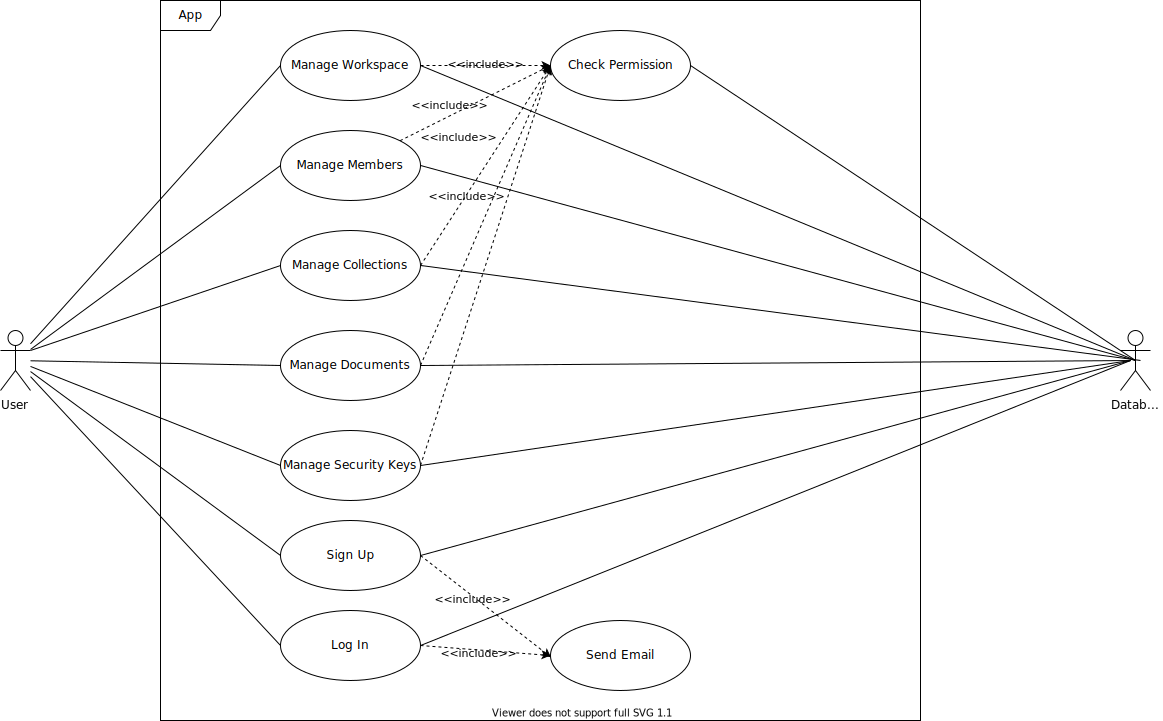
\includegraphics{./assets/UCD, General.svg}
%\caption{General use case diagram}
%\end{figure}

\hypertarget{conclusion-1}{%
\subsection{Conclusion}\label{conclusion-1}}

\emph{TBD}

\end{document}
